\section{Analytische Geometrie}
Die Analytische Geometrie ist eine Erweiterung der Analysis, um den dreidimensionalen Raum. Grundlegend wird in der Analytischen Geometrie im dreidimensionalen Raum gerechnet.
\subsection{Normen und Regeln}
In der Analytischen Geometrie gibt es Eigenschaften, die wichtig im Kopf zu behalten. 
\subsubsection{Zeichnen eines karthesischen Koordinatensystems}
Das Zeichnen eines karthesischen Koordinatensystems beginnt mit im Wesentlichen wie das Zeichnen eines zweidimensonalen Koordinatensystems.
\begin{itemize}
\item[1] Zuerst werden, wie bei einem zweidimensionalen Koordinatensystem, die beiden Achsen eingezeichnet. Hierbei ändert sich die Beschriftung der Achsen, da nun unsere ehemalige $x$-Achse die $y$-Achse ist und die ehemalige $y$-Achse nun die $z$-Achse.
\item[2] Anschließend nutzt man die Kästchen, die auf dem Blatt bereits vorgezeichnet sind und zeichnet in einem $45^{\circ}$. Dies bedeutet die $x$-Achse kommt aus dem Blatt heraus. 
\item[3] Nun kann an die nach oben zeigende Achse mit $z$, die horizontale Achse mit $y$ und die aus dem Blatt kommende mit $x$ beschriftet werden. 
\item[4] Die Skalierung der Achsen ist bei der $z$-Achse und der $y$-Achse gleich, wie bei einem zweidimensionalen Koordinatensystem. Die $x$-Achse hingegen nutzt die Hälfte einer relative Länge der Einheit auf der $z$ oder $y$-Achse. Dies bedeutet, dass ist eine Einheit auf der $y$-Achse in ein $cm$ skaliert ist die $1$ auf dieser bei einem Zentimeter. Auf der $x$-Achse ist sie bei $0.5cm$
\end{itemize}
Da das Zeichnen eines dreidimensionalen Koordiantensystems zeitintensiv ist, stellt die Website Kölzer eine Reihe an Vorlagen bereit, welche einfach in Dokumente importiert werden können. Ebenfalls stellt sie einen interaktiven Koordinatensystemgenerator zu verfügung, um Koordinatensystem in eigener Skalierung zu erstellen.\\
\link{https://kölzer.eu/koordinatensystem/}{Kölzer 3D-Plot}

Den Ablauf des Zeichnens wird ebenfalls durch das folgende Fliesdiagramm dargestellt. 
\includegraphics[width=9cm]{Algorithmen/karthesisches-Koordinatensystem-zeichen/karthesisches-Koordinatensystem-zeichen.drawio.pdf}
\subsection{Der dreidimensionale Raum}
Der dreidimensonale Raum wird beschrieben durch die 3 Achsen, die somit einem Punkt ermöglichen jede erdenkliche Position im Raum anzugeben. 


\subsection{Punkte einzeichnen}
Um einen Punkt in ein dreidimensonales Koordinatesystem einzuzeichen geht man wie folgt vor.
\begin{itemize}
	\item[1] Den im Punkt geben Wert auf der $x_1$-Achse gehen
	\item[2] Von dem vorherigen Schritt aus geht man nun in relativen Einheiten die Schritte, die als $x_2$-Achse oder $y$-Achse angeben sind. 
	\item[3] Abschließend geht man nun relative Einheiten auf der $x_3$-Achse  
\end{itemize} 

\subsection{Punkt bestimmen}
Um einen Punkt im Koordinatensystem zu bestimmen wird mindestens eine Koordinate benötigt, da sonst eine unendlich große Zahle an Möglichkeiten entstehet. Ist eine Koordinate bekannt, eines eingezeichneten Punktes, kann man sich Hilfslinien einzeichnen, die paralell zu den Koordinateneben verlaufen. 
\begin{itemize}  
\item[1] Projiziere Punkt $P$ mit Hilfe der bekannten Koordinate $K$ auf $P'(x,y,z)$ in die jeweilige Koordinatenebene $E$. (Gehe dafür vom Punkt $P$ aus $-K$ Einheiten in die jeweilige Koordinatenachse)  
\item[2] Zeichne vom projizierten Punkt p' aus Hilfslinien zu den Achsen, die die jeweilige Koordinatenebene E aufspannen. (Hilfslinien sind parallel zu den Koordinatenachsen der Ebene E)   
\item[3] Abschließend geht man nun relative Einheiten auf der $x_3$-Achse   
\end{itemize} 
\includegraphics[width=10cm]{Media/punktablesen3dKoordinatensystem.jpg}
\subsection{Spiegelung von Punkten}
Das spiegeln von Punkten in einem karthesischen Koordinatensystem erfordert immer die Voraussetzung, dass angegeben ist zu welcher Koordinatenebene ein Punkt gespiegelt werden soll. Um einen Punkt an einer Koordinatenebene zu spiegeln kann einfach das Vorzeichen der nicht betroffenen Koordinatenachse umkehren und erhält somit die Spiegelung. 
Der Punkt $A(3,4,5)$ soll an der $x_1/x_2$-Ebene gespiegelt werden. Da ein Punkt 
aus dem folgenden Triplet aus Koordinaten besteht, folgt also, dass wir das
Vorzeichen der Koordinate $x_3$ ändern müssen. 
$P(x_1,x_2,x_3)$
In der Anwendung von Differnetialgleichungen gibt es außerdem noch die
Möglichkeit Bedingungen aufzustellen ($f(0)=1$). Mit solchen Bedingungen kann
man wie folgt umgehen.

\begin{beispiel}
\begin{align*}
	A(3,4,5) \rightarrow B(3,4,-5)
\end{align*}
\end{beispiel}
\subsection{Vektor}
Ein Vektor ist eine Richtungsangabe im dreidimensonalen Raum. Sie werden in relativen Einheiten von ihrem Startpunkt aus angeben. 
\begin{figure}[h]
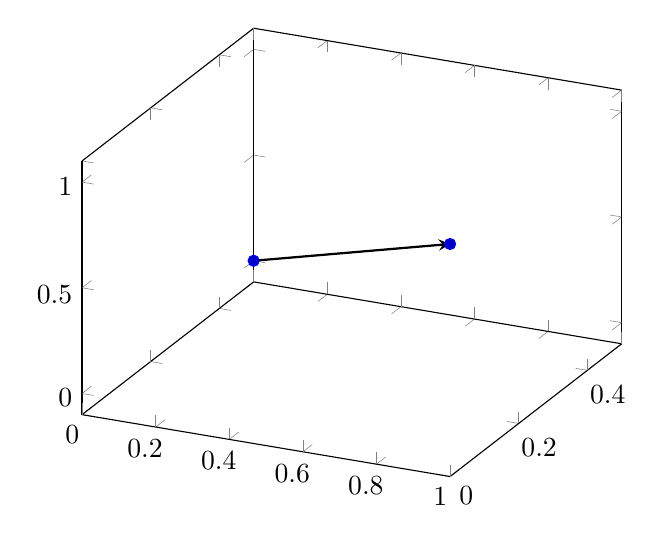
\begin{tikzpicture}
 \centering
\begin{axis}
 
\addplot3 coordinates 
{
    
    (0,0.5,0)
    (1,0,1)
    
};
\addplot3[no marks, -stealth, thick, black] coordinates {(0,0.5,0) (1,0,1)};
 
\end{axis}
 
\end{tikzpicture}

\end{figure}
\subsubsection{Notation}
Die Notation von Vektoren unterscheidet sich von der Angabe von Punkten deutlich, da sie die Koordianten übereinander darstellt. Wird ein Vektor zwischen zwei Punkten angeben, so besitzt dieser den Namen der beiden Punkte mit einem Pfeil über den Namen ($\vec{AB}$). 
\begin{align*}
\begin{pmatrix} x \\ y\\ z \end{pmatrix}
\end{align*}
\subsubsection{Nullvektor}
Der Nullvektor wird als solcher bezeichnet, da er der Vektor im Ursprung ist. Dieser besitzt die Koordinaten $\vec{0}=\begin{pmatrix} 0 \\ 0\\ 0 \end{pmatrix}$ Auch Punkte können als Vektor dargestellt werden, indem man man hierbei von dem Nullvektor zu dem Punkt verweißt. Ein solcher Punkt besitzt anschließend immer den Namen $\vec{OA}$, wobei $A$ der Punkt ist, auf den der Vektor zeigt.
\subsubsection{Gegenvektor}
Der Gegenvektor eines Vektor ist der Vektor, der in die entgegengesetzte Richtung zeigt. Besitzt ein Vektor also die Koordinaten 
$\vec{OA}=\begin{pmatrix}
	2\\3\\4
\end{pmatrix}$ $\rightarrow$ $\vec{OA}=\begin{pmatrix}
	-2\\-3\\-4
\end{pmatrix}$
\subsection{Punkt zu Vektor}
Bei einem Punkt, dessen Koordinaten angegeben sind, ist es möglich, dass dieser als Vektor angeben wird. Da Vektoren in relativen Einheiten angegeben werden, muss dies hierbei auch beachtet werden. Bei einem Punkt ist dies einfach, da man vom Ursprung ausgeht. Somit folgt, dass der Vektor exakt die selben Koordinaten wie der Punkt besitzt. 

\begin{beispiel}
	\begin{align*}
		A(2,3,4) \rightarrow \vec{OA}\begin{pmatrix}
			2\\3\\4
		\end{pmatrix}
	\end{align*}
\end{beispiel}
\pagebreak
\subsection{Länge eines Vektors}
Da Vektoren relativ zu einem anderen Punkt angeben sind besitzten diese auch eine Länge. Diese Länge kann berechnet werden durch den dreidimensonalen Satz des Phytagoras. Die Grundlage hierfür ist der Satz des Phytagoras, welcher $a^2+b^2=c^2$ lautet. Das Ziel bei dem dreidimensonalen Phytagoras das selbe Prinzip anzuwenden, jedoch mit der Besonderheit, dass er doppelt angewendet werden muss. Geht man davon aus, dass der Vektor $\vec{AB}$ berechnet werden soll und $A(a_1|a_2|a_2)$, $B(b_1|b_2|b_3)$ lauten, wobei ein Punkt folgendes Koordinatentripplet $P(x|y|z)$ besitzt,  sieht der dreidimensonale Satz des Phytagoras wie folgt aus. 
\begin{align*}
	|\vec{AB}|=\sqrt{(b_1-a_1)^2+(b_2-a_2)^2+(b_3-a_3)}
\end{align*}
Betrachtet man, was beim Anwenden passiert, fällt auf, dass durch das Subtrahieren von $b_1 - a_1$ die Differenz entsteht, und dies führt zu $a^2$ in der Normalform des Satzes des Pythagoras. Das Gleiche passiert beim zweiten Term. Wendet man nun den Satz des Pythagoras an, erhält man $\lvert \vec{AC} \rvert$ und hat somit die Grundlage für die zweite Anwendung des Satzes des Pythagoras ($a^2$). Addiert man nun $(\lvert \vec{AC} \rvert)^2$ mit $(\lvert \vec{CB} \rvert)^2$, so erhält man $(\lvert \vec{AB} \rvert)^2$. Zieht man die Wurzel, ergibt sich die Länge des Vektors $\vec{AB}$.

\begin{figure}[h]
\centering
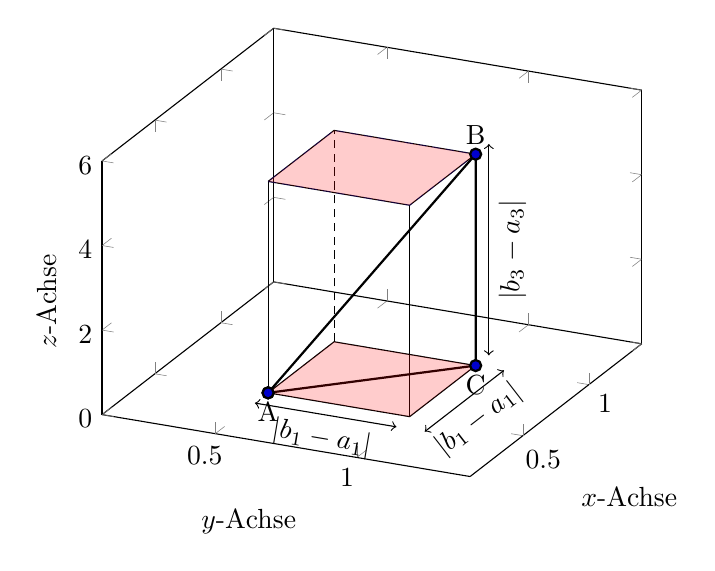
\begin{tikzpicture}
\begin{axis}[
	clip=false,
	xmin=0.1, xmax=1.4,
    ymin=0.1, ymax=1.4,
    zmin=0, zmax=6,
    xlabel={$y$-Achse},
    ylabel={$x$-Achse},
    zlabel={$z$-Achse},]
 
\addplot3+[black, thick] coordinates {
    (0.5,0.5,0)
    (1,1,5)
    (1,1,0)
    (0.5,0.5,0)
};  
\addplot3+[no markers, black] coordinates {(0.5,0.5,0) (1,0.5,0) (1,1,0) (0.5,1,0) (0.5,0.5,0)}; % Obere Fläche
\addplot3+[no markers, black] coordinates {(0.5,0.5,5) (1,0.5,5) (1,1,5) (0.5,1,5) (0.5,0.5,5)}; % Untere Fläche
\addplot3+[no markers, black] coordinates {(0.5,0.5,0) (0.5,0.5,5)}; % Vertikale Linien
\addplot3+[no markers, black] coordinates {(1,0.5,0) (1,0.5,5)};
\addplot3+[no markers, black] coordinates {(1,1,0) (1,1,5)};
\addplot3+[no markers, black] coordinates {(0.5,1,0) (0.5,1,5)};

\addplot3+[no markers, fill=red, opacity=0.2] coordinates {(0.5,0.5,0) (1,0.5,0) (1,1,0) (0.5,1,0) (0.5,0.5,0)}; % Obere Fläche
\addplot3+[no markers,fill=red, opacity=0.2] coordinates {(0.5,0.5,5) (1,0.5,5) (1,1,5) (0.5,1,5) (0.5,0.5,5)}; % Obere Fläche

\node at (axis cs:0.5,0.5,0) [anchor=north] {A};
\node at (axis cs:1,1,5) [anchor=south] {B};
\node at (axis cs:1,1,0) [anchor=north] {C};

\draw[<->] (axis cs:1,1.1,0) -- (axis cs:1,1.1,5) node[midway, sloped, below] {$|b_3-a_3|$};
\draw[<->] (axis cs:0.5,0.4,0) -- (axis cs:1,0.4,0) node[midway, sloped, below] {$|b_1-a_1|$};
\draw[<->] (axis cs:1.1,0.4,0) -- (axis cs:1.1,1,0) node[midway, sloped, below] {$|b_1-a_1|$};

\end{axis}
 
\end{tikzpicture}
\caption{Veranschaulichung des dreidimensonalen Satz des Phytagoras}
\end{figure}
\subsection{Skalarprodukt}
Das Skalarprodukt ist ein Produkt, welches durch eine Multiplikation eines mit einer Zahl mit dem Vektor entsteht. Das Multiplizieren erfolgt bei jeder Koordinate eines Vektors.
\subsection{Vektoren und Pfeile}
Vektoren können zur Beschreibung einer Verschiebung verwendet werden. Die Koordinaten de Vektors geben an, wie man bei der Verschiebung im Koordinatensystem von einem Punkt zu seinem Bildpunkt kommt. Verschiebungspfeile $\vec{TV}$, $\vec{RS}$ und $\vec{PQ}$ im Koordiantensystem rechts sind gleich gerichtet und gleichlang. Alle Pfeile veranschaulichen den gleichen Vektor. Umgekehrt bestimmt jeder Pfeil einen Vektor. So veranschaulicht etwa der Pfeil $\vec{PQ}$ von $P(6|4|1)$ nach $Q(10|3|4)$ den Vektor $\vec{v}$ mit $\vec{v}=\begin{pmatrix}
	10-6\\3-4\\4-1
\end{pmatrix}$
Man schreibt deshalb auch $\vec{PQ}=\begin{pmatrix}
	4\\-1\\3
\end{pmatrix}$. Dabei muss man beachten, dass der Vektor $\begin{pmatrix}
	4\\-1\\3
\end{pmatrix}$ zur Beschreibung der Verschiebung nicht an die Punkte $P$ und $Q$ gebunden ist. Er kann auch durch jeden anderen seiner Pfeile z.B. durch die Pfeile von $\vec{RS}$ oder von $\vec{TV}$, dargestellt werden. 
\begin{center}
	\includegraphics[width=6cm]{Media/VektorUndPunkt}
\end{center}



